In this chapter it is provided a brief introduction about the project described in the context of this essay.
\section{Medical Background}
The project focuses on the concept of \textbf{SNP}. SNP, \emph{Single Nucleotide Polymorphism}, is defined as a \emph{DNA sequence variation} occurring when a Single Nucleotide — A, T, C or G — in the genome (or other shared sequence) differs between members of a biological species or paired chromosomes. These variations can either be pathogenic, causing diseases, or completely harmless.
\\The main purpose for which the project is carried out is to \emph{help biologists understanding, having an ad-hoc organized database, when a particular SNP can cause diseases or not}.
\\The Web Portal allows them to \textbf{store} and \textbf{retrieve} Single Nucleotide Polymorphism genomics variants from a common database. This portal will then be used by biologists for this task, so it is realized so as to provide an intuitive and functional interface, which will act as an intermediary between the biologist and the actual database, facilitating their work as much as possible.
\\
\\The main functions of the portal are divided into two groups, depending on the privilege level of the user who use the system at the time:
\begin{description}
  \item[Super User] \hfill \\
  The \emph{Super User} is the user with the \emph{highest action privilege}, in fact it is in full possession of all the functionalities of the system.
\\As such, it can:
		\begin{itemize}
  		\item create a “family” with one or more members
 		 \item authorize users
 		 \item modify inserted values
		\end{itemize}
Basically, it can add, modify and enter the values it wants to. Obviously, the Super User can perform all the activities that Authorized User can do.
\\
  \item[Authorized User] \hfill \\
The \emph{Authorized User} is the one with a \emph{lower degree of privilege}, so it can not perform all the typical actions of the Super User, such as edit and insert. 
\\It only can:
		\begin{itemize}
  		\item search for a patient
		\item search for a gene
		\item search for a mutation
		\item \ldots
		\end{itemize}
The authorized user is someone who can query the portal, but who can not modify any values​​.
\\
\end{description}
The distinction between types of users has been designed to \emph{provide a control mechanism against unwanted anomalies}; in fact, if a biologist is interested in making simple queries to the system, he is able do it in a way that no changes or accidental deletions occurs.

\section{Project Structure}
We will now describe the structure of the project.
\\
\\The project is divided into three parts, which represent the basic structure of the portal:
\begin{enumerate}
  \item \textbf{Database}
  \item \textbf{Database - Website interaction}
  \item \textbf{Website (User Interface)}
\end{enumerate}

\subsection{Database}
The database is the most important part of the whole project, in fact the portal acts as an \emph{intermediary} between the database itself and the biologist. \textbf{All informations about the SNPs are stored in the database}. It follows that a poorly designed database can invalidate all the work related to the portal; therefore the good output of the same is conditioned first of all by a good design of the database.
\\
\\We will not focus on a detailed description of the structure of the database (that will be explained in \emph{Chapter 1}).
\\We can see, however, that the most important part of the database is represented by the concept of \textbf{variation}, which represents nothing more that \emph{a variation within the genome}. All other elements that need to be managed refer to the variant; we mention by way of example the gene relative to the variant, or the patient on which refers the same variant.
  
\subsection{Database - Website interaction}
Interaction between Database and Website is based on a \emph{series of queries}, that the user can send to the system to retrieve the information it wants. These queries are then executed on the database and the result returned to the user. 
\\
\\Items covered by those queries may be different; for example, the system allows searching for:
\begin{itemize}
 \item patient’s SNPs
 \item gene’s SNPs
 \item region’s SNPs
 \item all SNPs with certain Mutation, Genotype, Freq alt,\ldots
 \item patients with same SNP or Genotype
 \item SNPs within a genomic region
 \item specific SNP
 \item \ldots
\end{itemize}

The interactions can be carried out, as explained earlier, by all users (either Autenticated or Super User). The interactions for editing and adding data may relate to any entity in the database.

\subsection{Website (User Interface)}
The portal interface is represented by web pages, containing forms allowing to submit queries.
\\The fundamental characteristics that this interface must have are directly related to the it's purpose; we have to make sure that the biologists are facilitated as much as possible in their work of storing and retrieving information, to ensure that their work is as fast as possible. This affects also the intuitiveness and ease of use of the interface, that have to be taken into primary consideration.

\section{Use cases}
In this section we will discuss the use cases, illustrating the use of the system.
\\They will show how the user interacts with the system, from the point of view of the messages exchanged with it, and how the system handles these messages. You can see that the patterns of the use cases are similar to each other, since all gets the message from the user, and run it to the database by sending a special message for each request submitted.
\\
\\We will now analyse briefly each use case.
\subsection{Super User authorizes an User}
	\begin{figure}[ht!]
	\centering
	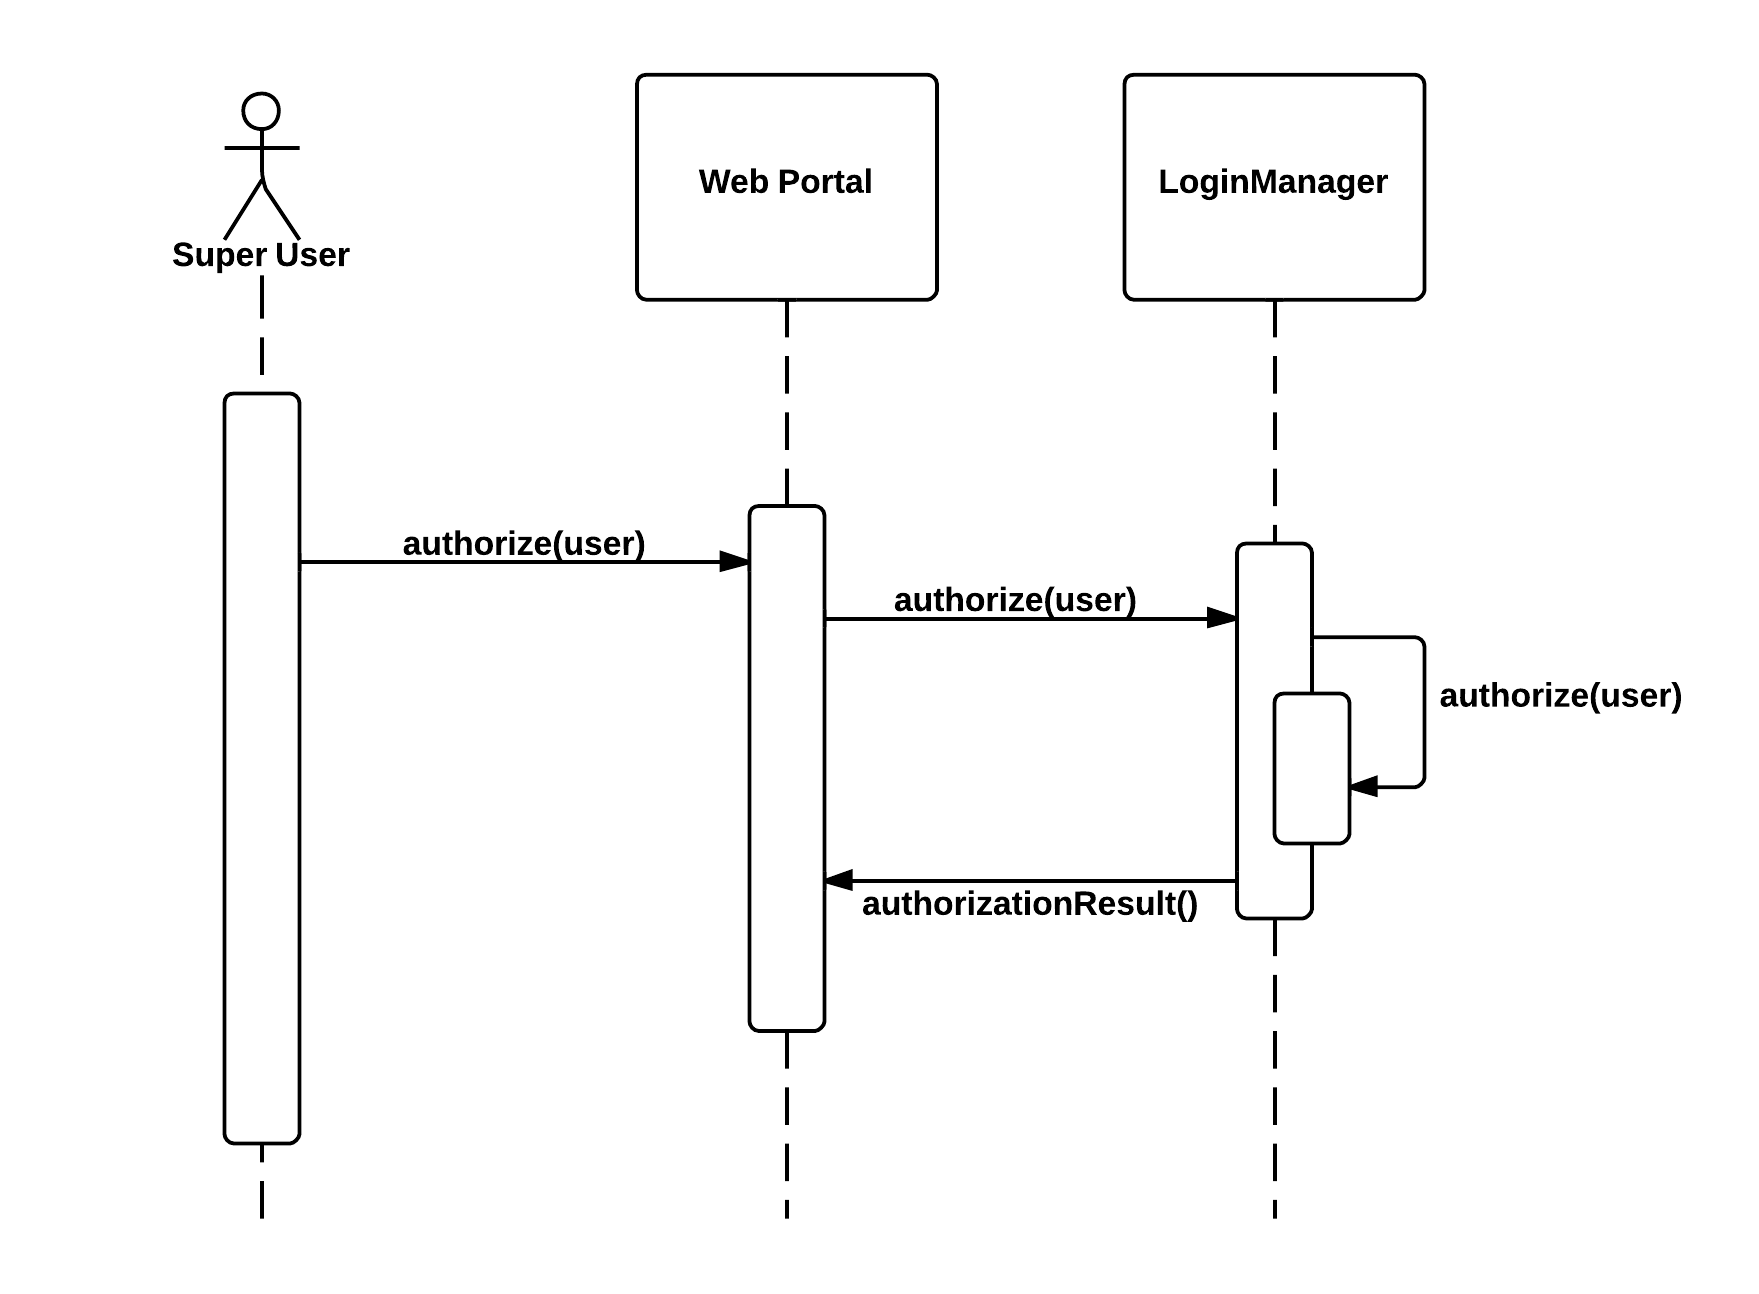
\includegraphics[width=90mm]{../Slides/images/Presentation_short_SSD_1.png}
	\label{overflow}
	\end{figure}
In this use case the actors are the \textbf{Super User}, the \textbf{Web Portal} and the \textbf{Login manager}.The user's intention is to allow another user to have privilege for using the portal.\\
\\The interaction begins with the super user that sends a message \emph{authorize(user)}to the Web portal. The latter sends the same message to the login manager, wich will be responsible to communicate with the database to record the granted permission. Successicely, the login manager sends a message to the web portal \emph{authorization(result)}, containing the result of the operation, so that the Web Portal can know whether the authorization was granted or not.

\subsection{Super User creates/populates a family}

In this use case the actors are the \textbf{Super User}, the \textbf{Web Portal} and the \textbf{Family DAO}. The user's intention is to create a new family, and populate it with a member. \\
\\The interaction starts with the user sending a message \emph{createFamily (familyID)} to Web Portal, which sends a message similar to FamilyDAO, the class responsible for managing / creating families and its interaction with the database. This class then communicates with the database itself, and sends a message containing the create result to the Web Portal. \\
\\If the family creation is successful, then the user can populate it, through a message  \emph{addMember(memberID)} sent to the Web Portal. The portal then dispatches the message to the FamilyDAO, who will add the member to the family, and returns the result to the Web Portal.

\begin{figure}[ht!]
	\centering
	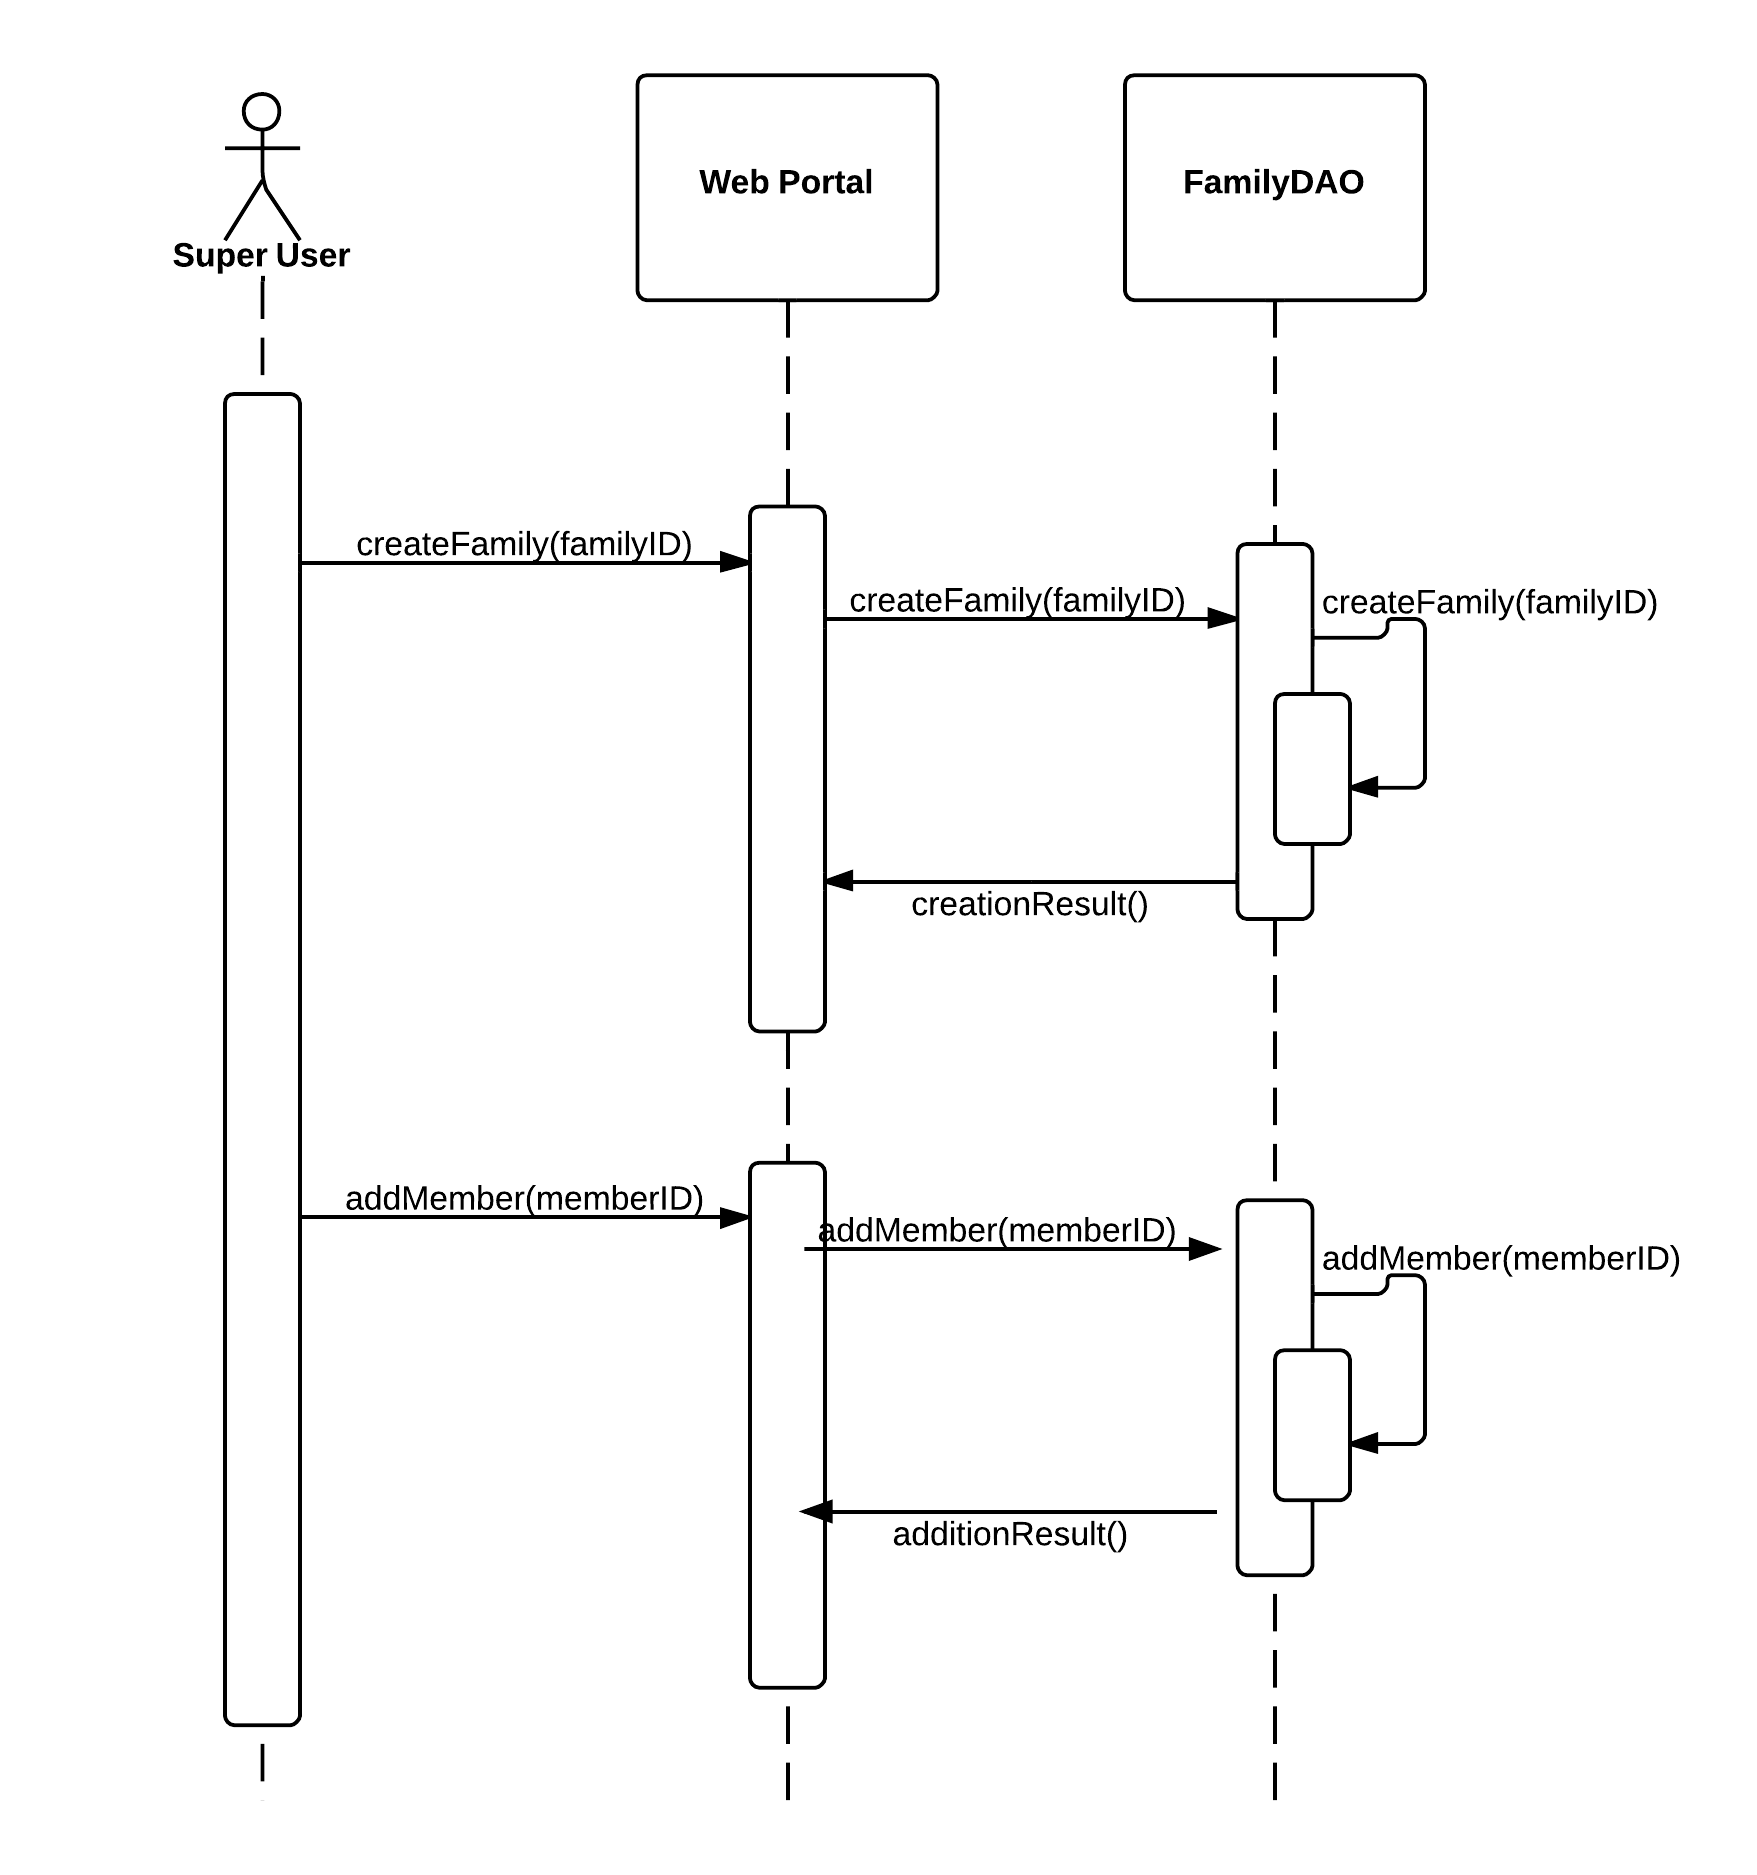
\includegraphics[width=90mm]{../Slides/images/Presentation_short_SSD_2.png}
	\label{overflow}
	\end{figure}
\subsection{Super User loads data}
	\begin{figure}[ht!]
	\centering
	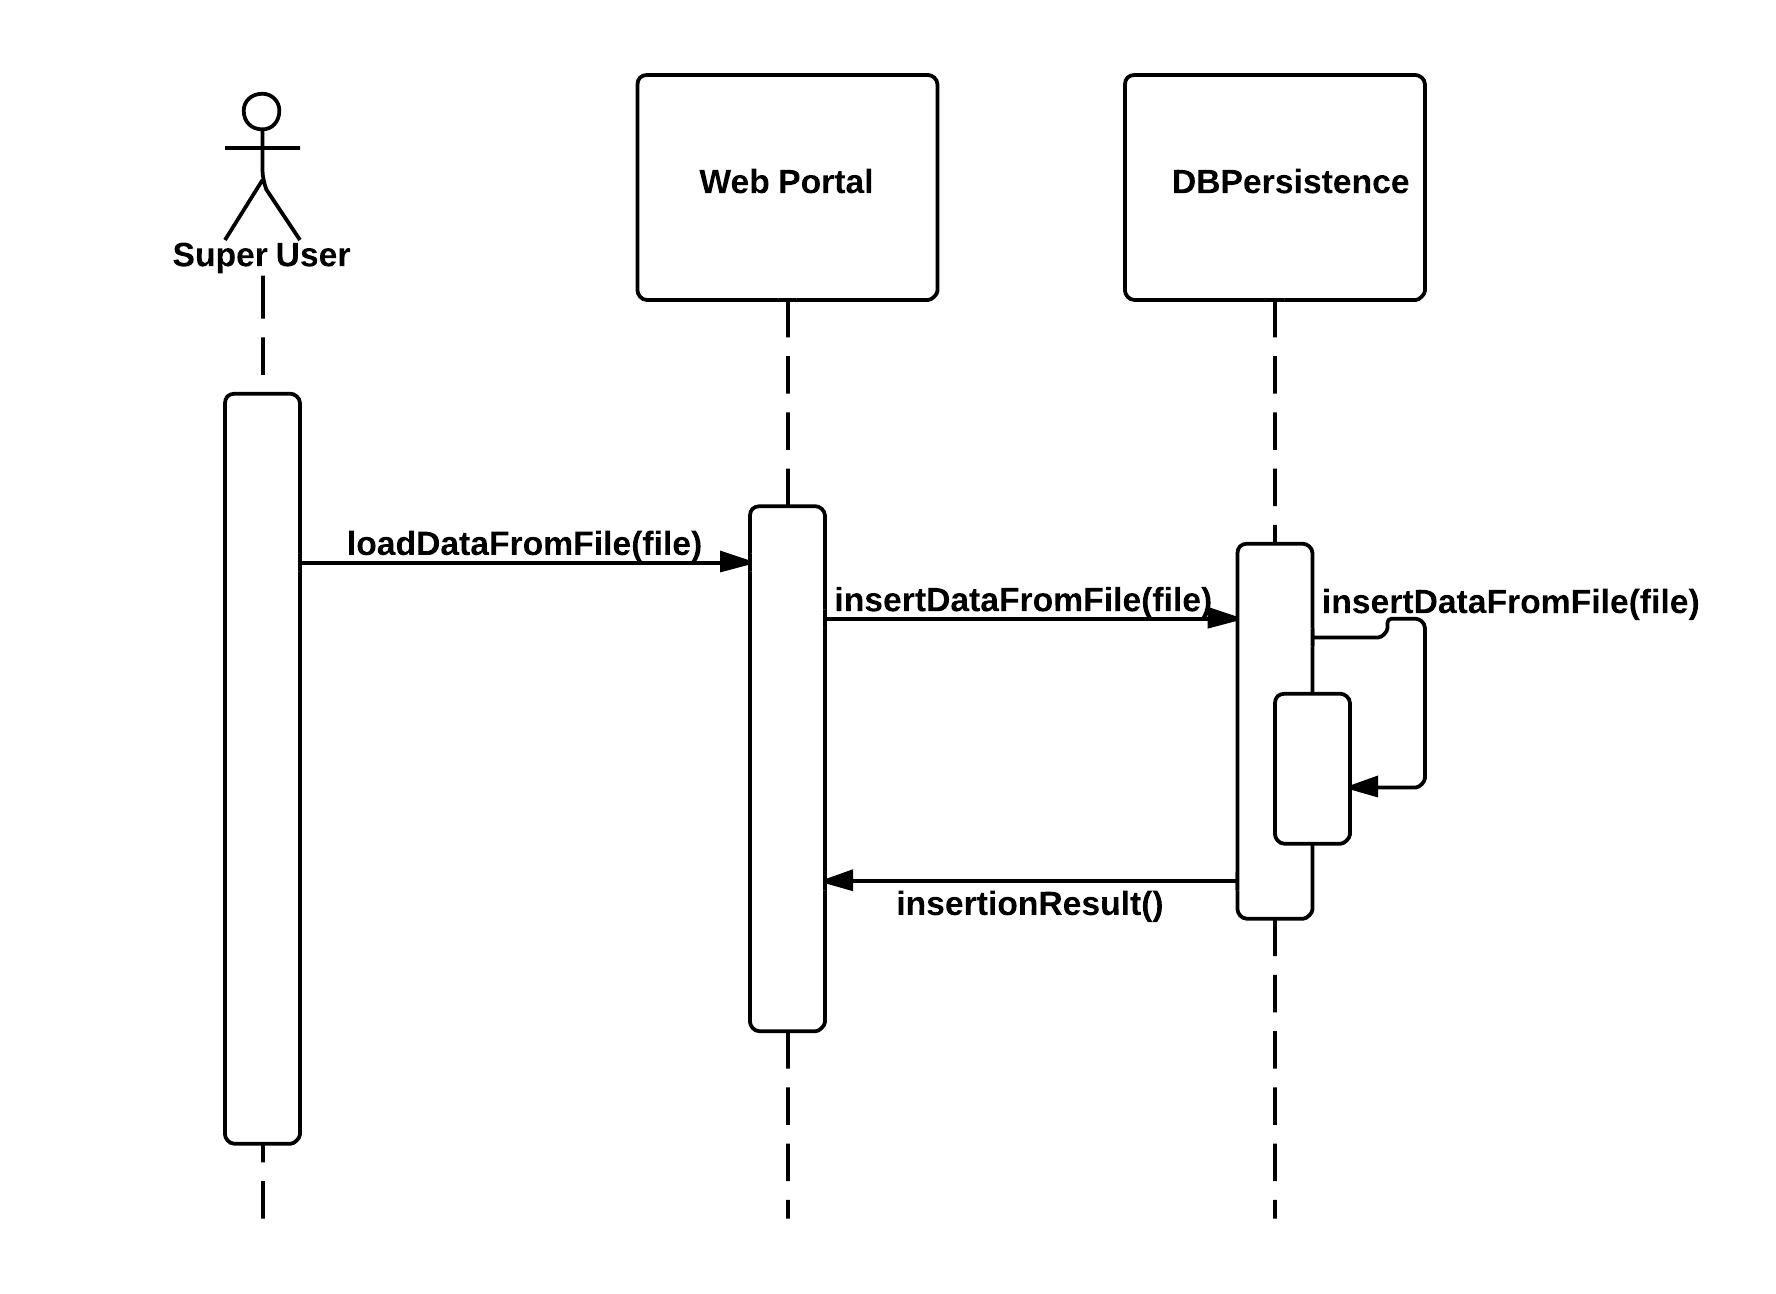
\includegraphics[width=90mm]{../Slides/images/Presentation_short_SSD_3.png}
	\label{overflow}
	\end{figure}
In this use case the actors are the \textbf{Super User}, the \textbf{Web Portal} and the \textbf{DBpersistence}. The user's intention is to load the data that have to be stored in the database, for later querying. Note that data is submitted to the system by using a comma-separated file. \\
\\To accomplish this task, the user sends a message to the web portal \emph{lodaDataFromFile(file)}, which file, as mentioned before, is a comma-separated file containing all the necessary data. Then the web portal sends message and data to the DBperistence class that both parse the file, and pass all information contained in file to the database, which will then store them. \\
\\Successively, this class will send the result of this insertion to the web portal through a message \emph{insertionResult()}.

\subsection{Authorized User executes a query}

In this use case the actors are the \textbf{Authorized User}, the \textbf{Web Portal} and the \textbf{QueryManager}. 
The user's intention is to run a query on the system, in order to obtain the information he wants to.\\
\\The user then sends a message \emph{query()} to the web portal, which will contain a generic query submitted by the user.The portal will send a message \emph{executeQuery()} to QueryManager, who will actually run the query in the database, and return the results to the portal. It does this through a message \emph{QueryResult()}

\begin{figure}[ht!]
	\centering
	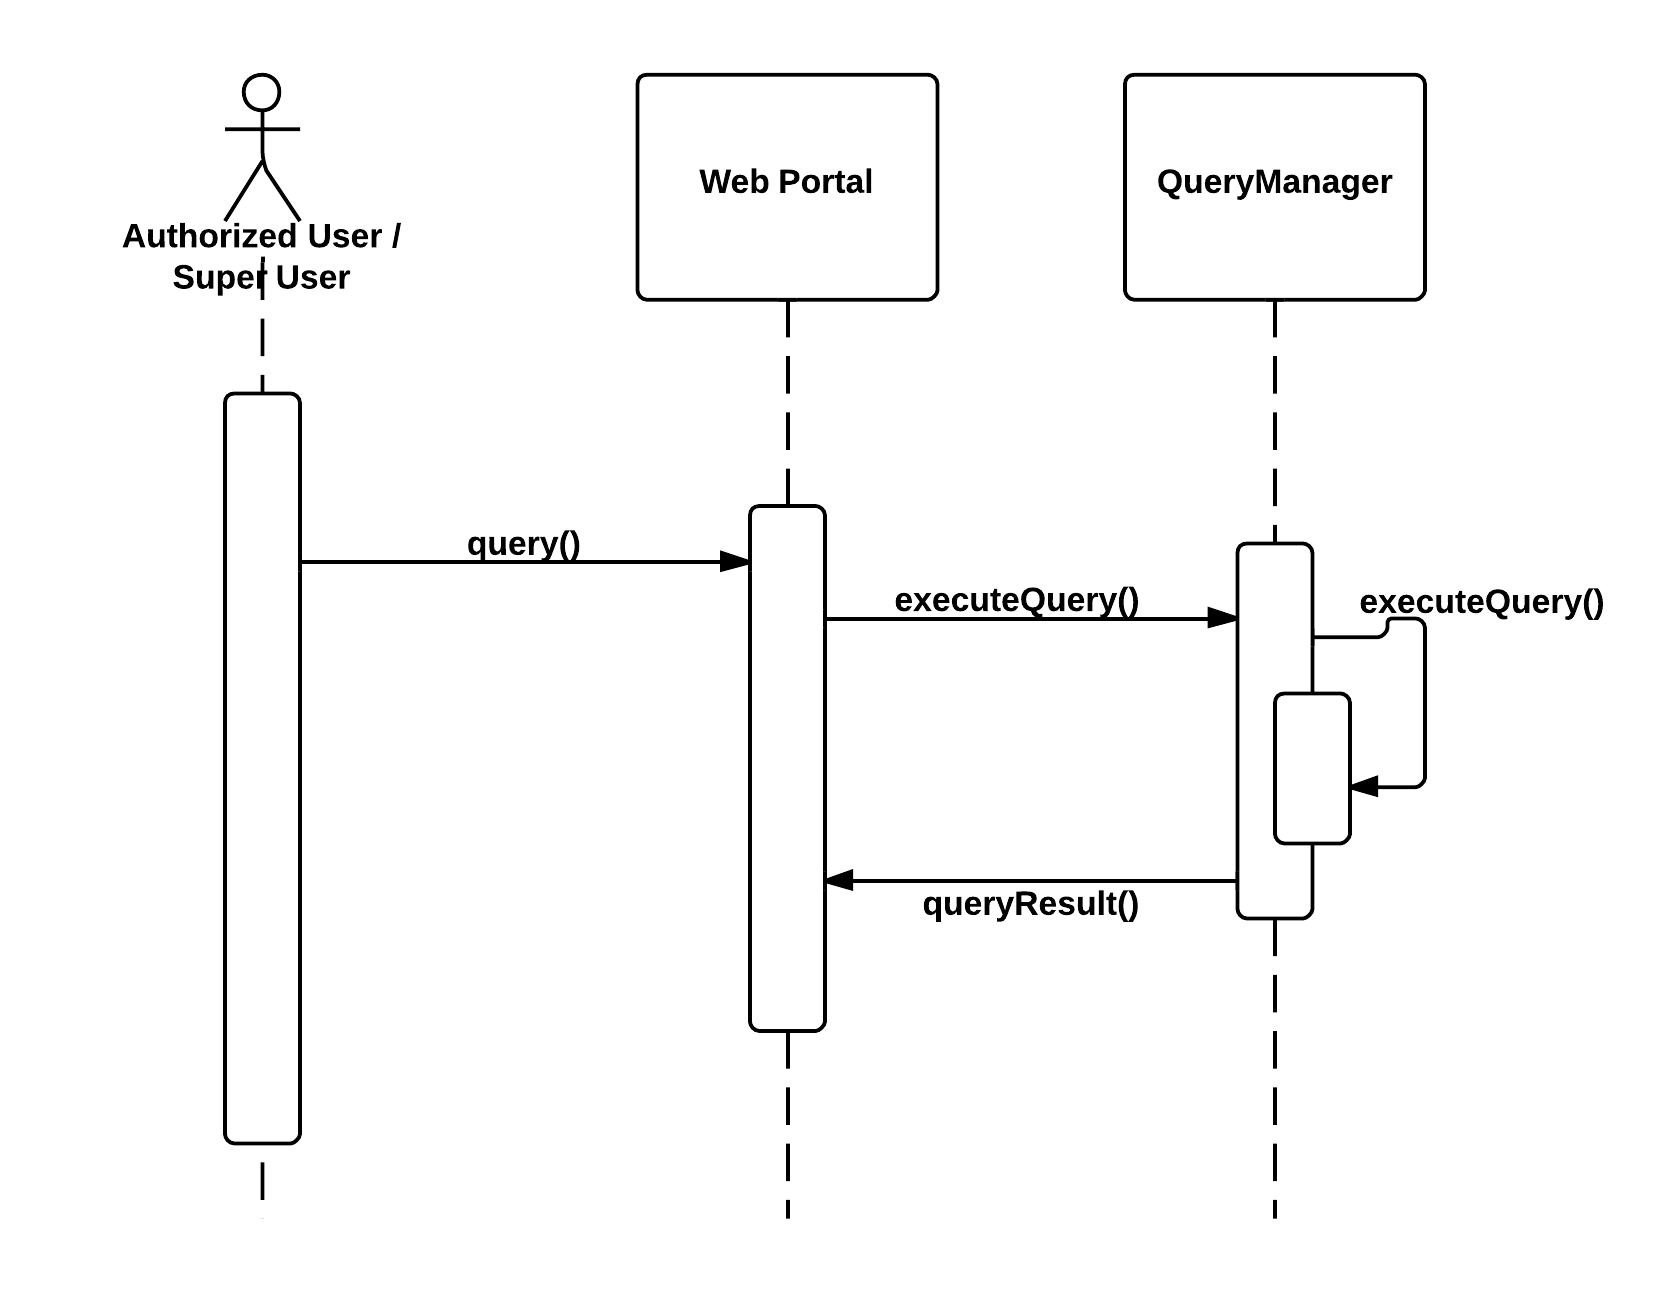
\includegraphics[width=90mm]{../Slides/images/Presentation_short_SSD_4.png}
	\label{overflow}
	\end{figure}

\section{Software architecture and tecnologies}
In this section we will discuss the software technologies used in the project, both for the front-end and back-end.
\subsection{Programming language}
The only programming language used throughout the project is \textbf{JavaScript}. This is because we want to use frameworks  supporting the JavaScript language (that can be considered one of the most utilised languages relating to dynamic content in web pages) that ensure a great rapidity of coding.

\newpage

\subsection{Technologies}
Technologies used all ri around chosen language. In particular:
\begin{description}
  \item[Database:] MongoDB
  \item[Website:] AngularJS
  \item[Model:] NodeJS
  \item[Framework:] ExpressJS
\end{description}
MongoDB is a \emph{NoSQL object-oriented DBMS}, which is based on the use of documents to represent objects. AngularJS allows to \emph{extend HTML with instructions for building dynamic web pages}. NodeJS is an \emph{event-driven, non-blocking network platform for building applications}. ExpressJS is a \emph{web application framework for NodeJS}, that extends some of its features, to make development faster.
\\
\\These four components form the so-called \textbf{MEAN} stack; it has been chosen for its scalability and for the quickness of development it can offer.